\item Dois discos $A$ e $B$ têm massa de \SI{1}{\kilogram} e \SI{2.5}{\kilogram}, respectivamente. Se eles deslizam sobre um plano horizontalmente liso com as velocidades mostradas, determine suas velocidades logo após o impacto.
O coeficiente de restituição entre os discos é $e=0.6$.

\import{sections/answers/}{answer-3}

\vspace{-1.8cm}
\begin{flushright}
	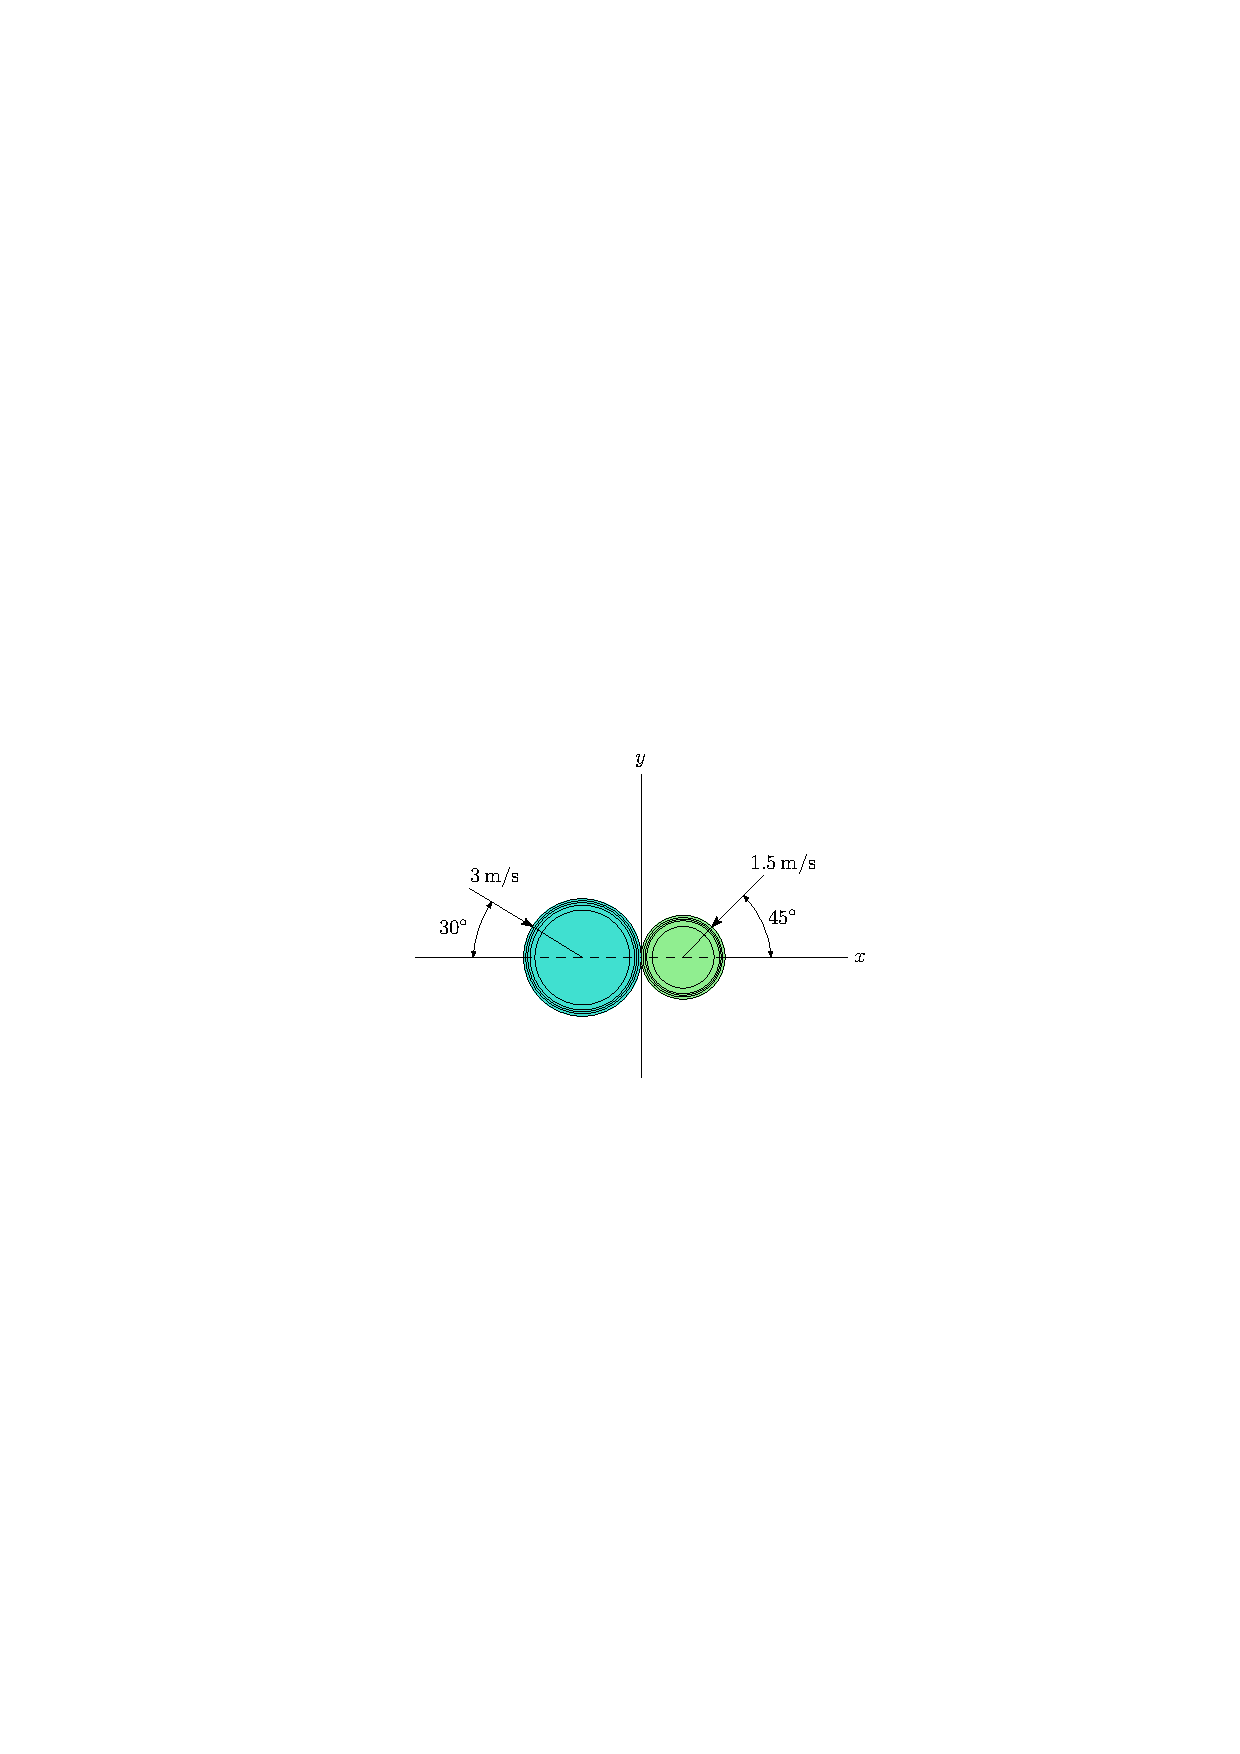
\includegraphics[scale=1.3]{images/draw_3}
\end{flushright}
\vspace{-1cm}